
\documentclass{acm_proc_article-sp}

%==================================
% packages go here
%==================================

\usepackage{url}
\usepackage{graphicx}
\usepackage{cite} % sort citation numbers
\usepackage{color}
\usepackage{soul}   
%\usepackage{ntheorem}
%\usepackage{amsthm}
%\usepackage{multirow} % for complex tables
%\usepackage{times}
%\usepackage[pdftex]{hyperref}
%\hypersetup{colorlinks=false, pdfborder= 0 0 0}
%\usepackage[draft,inline,nomargin]{fixme}
%\newcommand{\hlfixme}[1]{\fixme{\hl{#1}}}
%\newcommand{\hlfxnote}[1]{\fxnote{\hl{#1}}}

\newcommand{\name}{\emph{Watson Jr.}}

%==================================

\begin{document}

\title{Watson Jr.}
\subtitle{[A Question Answering System]}

\numberofauthors{3}
\author{
\alignauthor Name 1 \\
       \affaddr{University of Pittsburgh}\\
       \affaddr{Department of Computer Science}\\
       \email{email@domain.edu}
% author
\alignauthor Yann Le Gall\\
       \affaddr{University of Pittsburgh}\\
       \affaddr{Department of Computer Science}\\
       \email{ylegall@cs.pitt.edu}
% author
\alignauthor Name 3 \\
       \affaddr{University of Pittsburgh}\\
       \affaddr{Department of Computer Science}\\
       \email{email@domain.edu}
}

\date{12 December 2011}
\maketitle

%==================================

\begin{abstract}
abstract goes here
\end{abstract}

% A category with the (minimum) three required fields
\category{I.2}{Artifical Intelligence}{Natural Language Processing}
\terms{Algorithms, Experimentation}
\keywords{Question Answering}

%==================================

\section{Introduction}
\label{sec:intro}

In this paper, we design, implement, and evaluate a question answering
(QA) system. In our approach, we use several different strategies from
different domains to select potential answers. Then, we employ a
majority voting scheme to combine the results.

% TODO: should this description of the dataset go in another section?
To train and test our QA system, we used the ``CBC Reading
Comprehension Corpus''. This corpus is composed of 125 news stories,
each accompanied by a set of 6-10 factoid questions (e.g. questions
that begin with ``Who'', ``When'', ``Where'', etc.).
The news stories were obtained from the ``CBC 4 Kids'' website,
hosted by the Canadian Broadcast Corporation. The questions and an
answer key were added by the MITRE Corporation, and are in the style
of actual reading comprehension tests that are given to grade school
children in the United States.

All stories in the dataset were been split into sentences (one
sentence per line) using the MXTERMINATOR sentence splitter developed
by Adwait Ratnaparkhi.  Paragraphs from the original story are
separated by an empty line. 

The rest of this paper is organized as follows: in
\S\ref{sec:implementation} we describe the design and implementation
of our QA system and each of its sub-components. Next, in
\S\ref{sec:evaluation} we evaluate our system on the test dataset and
present the performance results. Finally, we conclude in
\S\ref{sec:conclusion}.


\section{Implementation}
\label{sec:implementation}

In this section we discuss the design and implementation of our QA
system. First, we explain the general, overall structure. Then we give
a detailed description of the sub-components (\emph{AnswerFinders}) of
the system . Finally, we present our technique for combining the
potential answers from each sub-component.

\begin{figure*} 
	\centering
	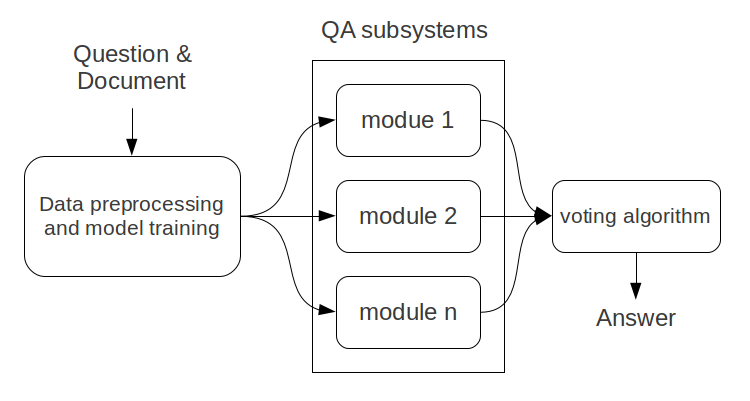
\includegraphics[width=0.8\textwidth]{model.png}
	\caption{The Watson Jr. system model.}
	\label{fig:model}
\end{figure*}

Figure \ref{fig:model} shows the general design of \name.
The system takes processes a document and a set of questions as input.
At this point, several preprocessing steps might be performed,
including the removal of stop words, coreference resolution, etc.
Next, the processed document and the current question are passed to
each of the AnswerFinders. Each of these AnswerFinders implements a
different strategy for finding answers to the question, and they
each return a collection of \texttt{<answer,confidence>} pairs.
Finally, the potential answers are combineded in a voting algorithm
that gives different weights to the potential answers based on the
confidence and the question type.

In the next few subsections, we give more detailed descriptions of
the implementation of the different AnswerFinders and the
strategies that they use.

\subsection{Bag-of-Words}

The Bag-of-words (BOW) model is a simple model that provides relatively good
performance in our systeml. In our domain, BOW treats each question as
a set of words. Then, for each sentence in the document, we count the
number of matching words. The sentence with the largest number of
matching words is chosen as the answer.

\subsection{Linguistic Rule-based Strategies}

% TODO: Yann writes this

\subsection{NLP Components}

% TODO: Alex writes this

\subsection{SVM Classification}

% TODO: Eric writes this part

\subsection{Combining Answers with Majority Voting}
Previous work by Rotaru and Litman demonstrates that combining
the outputs of multiple QA systems can achieve better results than the
individual systems alone \cite{rotaru2005}. We incorporate this idea
into the design of our QA system by combining the outputs from each of
the subsystems described above.

% TODO: describe how we combine the different results

\section{Evaluation}
\label{sec:evaluation}



\section{Conclusions}
\label{sec:conclusion}

Question-answering is complex task and a cutting-edge research area
in natural language processing. 


%ACKNOWLEDGMENTS are optional
%\section{Acknowledgments}

%\bibliographystyle{abbrv}
\bibliographystyle{plain}
\bibliography{references} 

%
%\appendix
%%Appendix A
%\section{Headings in Appendices}
%\balancecolumns


\end{document}

